\documentclass{article}

\usepackage{style/conference}
\usepackage{opensans}
\usepackage{graphicx}
\usepackage{biblatex}
\usepackage{fontawesome}
\usepackage[hidelinks]{hyperref}
\usepackage{floatrow}

\floatsetup[table]{capposition=top}
\floatsetup[figure]{capposition=top}

\newcommand{\norm}[1]{\left\lVert#1\right\rVert}

\addbibresource{references.bib}
%%%%% NEW MATH DEFINITIONS %%%%%

\usepackage{amsmath,amsfonts,bm}

% Mark sections of captions for referring to divisions of figures
\newcommand{\figleft}{{\em (Left)}}
\newcommand{\figcenter}{{\em (Center)}}
\newcommand{\figright}{{\em (Right)}}
\newcommand{\figtop}{{\em (Top)}}
\newcommand{\figbottom}{{\em (Bottom)}}
\newcommand{\captiona}{{\em (a)}}
\newcommand{\captionb}{{\em (b)}}
\newcommand{\captionc}{{\em (c)}}
\newcommand{\captiond}{{\em (d)}}

% Highlight a newly defined term
\newcommand{\newterm}[1]{{\bf #1}}


% Figure reference, lower-case.
\def\figref#1{figure~\ref{#1}}
% Figure reference, capital. For start of sentence
\def\Figref#1{Figure~\ref{#1}}
\def\twofigref#1#2{figures \ref{#1} and \ref{#2}}
\def\quadfigref#1#2#3#4{figures \ref{#1}, \ref{#2}, \ref{#3} and \ref{#4}}
% Section reference, lower-case.
\def\secref#1{section~\ref{#1}}
% Section reference, capital.
\def\Secref#1{Section~\ref{#1}}
% Reference to two sections.
\def\twosecrefs#1#2{sections \ref{#1} and \ref{#2}}
% Reference to three sections.
\def\secrefs#1#2#3{sections \ref{#1}, \ref{#2} and \ref{#3}}
% Reference to an equation, lower-case.
\def\eqref#1{equation~\ref{#1}}
% Reference to an equation, upper case
\def\Eqref#1{Equation~\ref{#1}}
% A raw reference to an equation---avoid using if possible
\def\plaineqref#1{\ref{#1}}
% Reference to a chapter, lower-case.
\def\chapref#1{chapter~\ref{#1}}
% Reference to an equation, upper case.
\def\Chapref#1{Chapter~\ref{#1}}
% Reference to a range of chapters
\def\rangechapref#1#2{chapters\ref{#1}--\ref{#2}}
% Reference to an algorithm, lower-case.
\def\algref#1{algorithm~\ref{#1}}
% Reference to an algorithm, upper case.
\def\Algref#1{Algorithm~\ref{#1}}
\def\twoalgref#1#2{algorithms \ref{#1} and \ref{#2}}
\def\Twoalgref#1#2{Algorithms \ref{#1} and \ref{#2}}
% Reference to a part, lower case
\def\partref#1{part~\ref{#1}}
% Reference to a part, upper case
\def\Partref#1{Part~\ref{#1}}
\def\twopartref#1#2{parts \ref{#1} and \ref{#2}}

\def\ceil#1{\lceil #1 \rceil}
\def\floor#1{\lfloor #1 \rfloor}
\def\1{\bm{1}}
\newcommand{\train}{\mathcal{D}}
\newcommand{\valid}{\mathcal{D_{\mathrm{valid}}}}
\newcommand{\test}{\mathcal{D_{\mathrm{test}}}}

\def\eps{{\epsilon}}


% Random variables
\def\reta{{\textnormal{$\eta$}}}
\def\ra{{\textnormal{a}}}
\def\rb{{\textnormal{b}}}
\def\rc{{\textnormal{c}}}
\def\rd{{\textnormal{d}}}
\def\re{{\textnormal{e}}}
\def\rf{{\textnormal{f}}}
\def\rg{{\textnormal{g}}}
\def\rh{{\textnormal{h}}}
\def\ri{{\textnormal{i}}}
\def\rj{{\textnormal{j}}}
\def\rk{{\textnormal{k}}}
\def\rl{{\textnormal{l}}}
% rm is already a command, just don't name any random variables m
\def\rn{{\textnormal{n}}}
\def\ro{{\textnormal{o}}}
\def\rp{{\textnormal{p}}}
\def\rq{{\textnormal{q}}}
\def\rr{{\textnormal{r}}}
\def\rs{{\textnormal{s}}}
\def\rt{{\textnormal{t}}}
\def\ru{{\textnormal{u}}}
\def\rv{{\textnormal{v}}}
\def\rw{{\textnormal{w}}}
\def\rx{{\textnormal{x}}}
\def\ry{{\textnormal{y}}}
\def\rz{{\textnormal{z}}}

% Random vectors
\def\rvepsilon{{\mathbf{\epsilon}}}
\def\rvtheta{{\mathbf{\theta}}}
\def\rva{{\mathbf{a}}}
\def\rvb{{\mathbf{b}}}
\def\rvc{{\mathbf{c}}}
\def\rvd{{\mathbf{d}}}
\def\rve{{\mathbf{e}}}
\def\rvf{{\mathbf{f}}}
\def\rvg{{\mathbf{g}}}
\def\rvh{{\mathbf{h}}}
\def\rvu{{\mathbf{i}}}
\def\rvj{{\mathbf{j}}}
\def\rvk{{\mathbf{k}}}
\def\rvl{{\mathbf{l}}}
\def\rvm{{\mathbf{m}}}
\def\rvn{{\mathbf{n}}}
\def\rvo{{\mathbf{o}}}
\def\rvp{{\mathbf{p}}}
\def\rvq{{\mathbf{q}}}
\def\rvr{{\mathbf{r}}}
\def\rvs{{\mathbf{s}}}
\def\rvt{{\mathbf{t}}}
\def\rvu{{\mathbf{u}}}
\def\rvv{{\mathbf{v}}}
\def\rvw{{\mathbf{w}}}
\def\rvx{{\mathbf{x}}}
\def\rvy{{\mathbf{y}}}
\def\rvz{{\mathbf{z}}}

% Elements of random vectors
\def\erva{{\textnormal{a}}}
\def\ervb{{\textnormal{b}}}
\def\ervc{{\textnormal{c}}}
\def\ervd{{\textnormal{d}}}
\def\erve{{\textnormal{e}}}
\def\ervf{{\textnormal{f}}}
\def\ervg{{\textnormal{g}}}
\def\ervh{{\textnormal{h}}}
\def\ervi{{\textnormal{i}}}
\def\ervj{{\textnormal{j}}}
\def\ervk{{\textnormal{k}}}
\def\ervl{{\textnormal{l}}}
\def\ervm{{\textnormal{m}}}
\def\ervn{{\textnormal{n}}}
\def\ervo{{\textnormal{o}}}
\def\ervp{{\textnormal{p}}}
\def\ervq{{\textnormal{q}}}
\def\ervr{{\textnormal{r}}}
\def\ervs{{\textnormal{s}}}
\def\ervt{{\textnormal{t}}}
\def\ervu{{\textnormal{u}}}
\def\ervv{{\textnormal{v}}}
\def\ervw{{\textnormal{w}}}
\def\ervx{{\textnormal{x}}}
\def\ervy{{\textnormal{y}}}
\def\ervz{{\textnormal{z}}}

% Random matrices
\def\rmA{{\mathbf{A}}}
\def\rmB{{\mathbf{B}}}
\def\rmC{{\mathbf{C}}}
\def\rmD{{\mathbf{D}}}
\def\rmE{{\mathbf{E}}}
\def\rmF{{\mathbf{F}}}
\def\rmG{{\mathbf{G}}}
\def\rmH{{\mathbf{H}}}
\def\rmI{{\mathbf{I}}}
\def\rmJ{{\mathbf{J}}}
\def\rmK{{\mathbf{K}}}
\def\rmL{{\mathbf{L}}}
\def\rmM{{\mathbf{M}}}
\def\rmN{{\mathbf{N}}}
\def\rmO{{\mathbf{O}}}
\def\rmP{{\mathbf{P}}}
\def\rmQ{{\mathbf{Q}}}
\def\rmR{{\mathbf{R}}}
\def\rmS{{\mathbf{S}}}
\def\rmT{{\mathbf{T}}}
\def\rmU{{\mathbf{U}}}
\def\rmV{{\mathbf{V}}}
\def\rmW{{\mathbf{W}}}
\def\rmX{{\mathbf{X}}}
\def\rmY{{\mathbf{Y}}}
\def\rmZ{{\mathbf{Z}}}

% Elements of random matrices
\def\ermA{{\textnormal{A}}}
\def\ermB{{\textnormal{B}}}
\def\ermC{{\textnormal{C}}}
\def\ermD{{\textnormal{D}}}
\def\ermE{{\textnormal{E}}}
\def\ermF{{\textnormal{F}}}
\def\ermG{{\textnormal{G}}}
\def\ermH{{\textnormal{H}}}
\def\ermI{{\textnormal{I}}}
\def\ermJ{{\textnormal{J}}}
\def\ermK{{\textnormal{K}}}
\def\ermL{{\textnormal{L}}}
\def\ermM{{\textnormal{M}}}
\def\ermN{{\textnormal{N}}}
\def\ermO{{\textnormal{O}}}
\def\ermP{{\textnormal{P}}}
\def\ermQ{{\textnormal{Q}}}
\def\ermR{{\textnormal{R}}}
\def\ermS{{\textnormal{S}}}
\def\ermT{{\textnormal{T}}}
\def\ermU{{\textnormal{U}}}
\def\ermV{{\textnormal{V}}}
\def\ermW{{\textnormal{W}}}
\def\ermX{{\textnormal{X}}}
\def\ermY{{\textnormal{Y}}}
\def\ermZ{{\textnormal{Z}}}

% Vectors
\def\vzero{{\bm{0}}}
\def\vone{{\bm{1}}}
\def\vmu{{\bm{\mu}}}
\def\vtheta{{\bm{\theta}}}
\def\va{{\bm{a}}}
\def\vb{{\bm{b}}}
\def\vc{{\bm{c}}}
\def\vd{{\bm{d}}}
\def\ve{{\bm{e}}}
\def\vf{{\bm{f}}}
\def\vg{{\bm{g}}}
\def\vh{{\bm{h}}}
\def\vi{{\bm{i}}}
\def\vj{{\bm{j}}}
\def\vk{{\bm{k}}}
\def\vl{{\bm{l}}}
\def\vm{{\bm{m}}}
\def\vn{{\bm{n}}}
\def\vo{{\bm{o}}}
\def\vp{{\bm{p}}}
\def\vq{{\bm{q}}}
\def\vr{{\bm{r}}}
\def\vs{{\bm{s}}}
\def\vt{{\bm{t}}}
\def\vu{{\bm{u}}}
\def\vv{{\bm{v}}}
\def\vw{{\bm{w}}}
\def\vx{{\bm{x}}}
\def\vy{{\bm{y}}}
\def\vz{{\bm{z}}}

% Elements of vectors
\def\evalpha{{\alpha}}
\def\evbeta{{\beta}}
\def\evepsilon{{\epsilon}}
\def\evlambda{{\lambda}}
\def\evomega{{\omega}}
\def\evmu{{\mu}}
\def\evpsi{{\psi}}
\def\evsigma{{\sigma}}
\def\evtheta{{\theta}}
\def\eva{{a}}
\def\evb{{b}}
\def\evc{{c}}
\def\evd{{d}}
\def\eve{{e}}
\def\evf{{f}}
\def\evg{{g}}
\def\evh{{h}}
\def\evi{{i}}
\def\evj{{j}}
\def\evk{{k}}
\def\evl{{l}}
\def\evm{{m}}
\def\evn{{n}}
\def\evo{{o}}
\def\evp{{p}}
\def\evq{{q}}
\def\evr{{r}}
\def\evs{{s}}
\def\evt{{t}}
\def\evu{{u}}
\def\evv{{v}}
\def\evw{{w}}
\def\evx{{x}}
\def\evy{{y}}
\def\evz{{z}}

% Matrix
\def\mA{{\bm{A}}}
\def\mB{{\bm{B}}}
\def\mC{{\bm{C}}}
\def\mD{{\bm{D}}}
\def\mE{{\bm{E}}}
\def\mF{{\bm{F}}}
\def\mG{{\bm{G}}}
\def\mH{{\bm{H}}}
\def\mI{{\bm{I}}}
\def\mJ{{\bm{J}}}
\def\mK{{\bm{K}}}
\def\mL{{\bm{L}}}
\def\mM{{\bm{M}}}
\def\mN{{\bm{N}}}
\def\mO{{\bm{O}}}
\def\mP{{\bm{P}}}
\def\mQ{{\bm{Q}}}
\def\mR{{\bm{R}}}
\def\mS{{\bm{S}}}
\def\mT{{\bm{T}}}
\def\mU{{\bm{U}}}
\def\mV{{\bm{V}}}
\def\mW{{\bm{W}}}
\def\mX{{\bm{X}}}
\def\mY{{\bm{Y}}}
\def\mZ{{\bm{Z}}}
\def\mBeta{{\bm{\beta}}}
\def\mPhi{{\bm{\Phi}}}
\def\mLambda{{\bm{\Lambda}}}
\def\mSigma{{\bm{\Sigma}}}

% Tensor
\DeclareMathAlphabet{\mathsfit}{\encodingdefault}{\sfdefault}{m}{sl}
\SetMathAlphabet{\mathsfit}{bold}{\encodingdefault}{\sfdefault}{bx}{n}
\newcommand{\tens}[1]{\bm{\mathsfit{#1}}}
\def\tA{{\tens{A}}}
\def\tB{{\tens{B}}}
\def\tC{{\tens{C}}}
\def\tD{{\tens{D}}}
\def\tE{{\tens{E}}}
\def\tF{{\tens{F}}}
\def\tG{{\tens{G}}}
\def\tH{{\tens{H}}}
\def\tI{{\tens{I}}}
\def\tJ{{\tens{J}}}
\def\tK{{\tens{K}}}
\def\tL{{\tens{L}}}
\def\tM{{\tens{M}}}
\def\tN{{\tens{N}}}
\def\tO{{\tens{O}}}
\def\tP{{\tens{P}}}
\def\tQ{{\tens{Q}}}
\def\tR{{\tens{R}}}
\def\tS{{\tens{S}}}
\def\tT{{\tens{T}}}
\def\tU{{\tens{U}}}
\def\tV{{\tens{V}}}
\def\tW{{\tens{W}}}
\def\tX{{\tens{X}}}
\def\tY{{\tens{Y}}}
\def\tZ{{\tens{Z}}}


% Graph
\def\gA{{\mathcal{A}}}
\def\gB{{\mathcal{B}}}
\def\gC{{\mathcal{C}}}
\def\gD{{\mathcal{D}}}
\def\gE{{\mathcal{E}}}
\def\gF{{\mathcal{F}}}
\def\gG{{\mathcal{G}}}
\def\gH{{\mathcal{H}}}
\def\gI{{\mathcal{I}}}
\def\gJ{{\mathcal{J}}}
\def\gK{{\mathcal{K}}}
\def\gL{{\mathcal{L}}}
\def\gM{{\mathcal{M}}}
\def\gN{{\mathcal{N}}}
\def\gO{{\mathcal{O}}}
\def\gP{{\mathcal{P}}}
\def\gQ{{\mathcal{Q}}}
\def\gR{{\mathcal{R}}}
\def\gS{{\mathcal{S}}}
\def\gT{{\mathcal{T}}}
\def\gU{{\mathcal{U}}}
\def\gV{{\mathcal{V}}}
\def\gW{{\mathcal{W}}}
\def\gX{{\mathcal{X}}}
\def\gY{{\mathcal{Y}}}
\def\gZ{{\mathcal{Z}}}

% Sets
\def\sA{{\mathbb{A}}}
\def\sB{{\mathbb{B}}}
\def\sC{{\mathbb{C}}}
\def\sD{{\mathbb{D}}}
% Don't use a set called E, because this would be the same as our symbol
% for expectation.
\def\sF{{\mathbb{F}}}
\def\sG{{\mathbb{G}}}
\def\sH{{\mathbb{H}}}
\def\sI{{\mathbb{I}}}
\def\sJ{{\mathbb{J}}}
\def\sK{{\mathbb{K}}}
\def\sL{{\mathbb{L}}}
\def\sM{{\mathbb{M}}}
\def\sN{{\mathbb{N}}}
\def\sO{{\mathbb{O}}}
\def\sP{{\mathbb{P}}}
\def\sQ{{\mathbb{Q}}}
\def\sR{{\mathbb{R}}}
\def\sS{{\mathbb{S}}}
\def\sT{{\mathbb{T}}}
\def\sU{{\mathbb{U}}}
\def\sV{{\mathbb{V}}}
\def\sW{{\mathbb{W}}}
\def\sX{{\mathbb{X}}}
\def\sY{{\mathbb{Y}}}
\def\sZ{{\mathbb{Z}}}

% Entries of a matrix
\def\emLambda{{\Lambda}}
\def\emA{{A}}
\def\emB{{B}}
\def\emC{{C}}
\def\emD{{D}}
\def\emE{{E}}
\def\emF{{F}}
\def\emG{{G}}
\def\emH{{H}}
\def\emI{{I}}
\def\emJ{{J}}
\def\emK{{K}}
\def\emL{{L}}
\def\emM{{M}}
\def\emN{{N}}
\def\emO{{O}}
\def\emP{{P}}
\def\emQ{{Q}}
\def\emR{{R}}
\def\emS{{S}}
\def\emT{{T}}
\def\emU{{U}}
\def\emV{{V}}
\def\emW{{W}}
\def\emX{{X}}
\def\emY{{Y}}
\def\emZ{{Z}}
\def\emSigma{{\Sigma}}

% entries of a tensor
% Same font as tensor, without \bm wrapper
\newcommand{\etens}[1]{\mathsfit{#1}}
\def\etLambda{{\etens{\Lambda}}}
\def\etA{{\etens{A}}}
\def\etB{{\etens{B}}}
\def\etC{{\etens{C}}}
\def\etD{{\etens{D}}}
\def\etE{{\etens{E}}}
\def\etF{{\etens{F}}}
\def\etG{{\etens{G}}}
\def\etH{{\etens{H}}}
\def\etI{{\etens{I}}}
\def\etJ{{\etens{J}}}
\def\etK{{\etens{K}}}
\def\etL{{\etens{L}}}
\def\etM{{\etens{M}}}
\def\etN{{\etens{N}}}
\def\etO{{\etens{O}}}
\def\etP{{\etens{P}}}
\def\etQ{{\etens{Q}}}
\def\etR{{\etens{R}}}
\def\etS{{\etens{S}}}
\def\etT{{\etens{T}}}
\def\etU{{\etens{U}}}
\def\etV{{\etens{V}}}
\def\etW{{\etens{W}}}
\def\etX{{\etens{X}}}
\def\etY{{\etens{Y}}}
\def\etZ{{\etens{Z}}}

% The true underlying data generating distribution
\newcommand{\pdata}{p_{\rm{data}}}
% The empirical distribution defined by the training set
\newcommand{\ptrain}{\hat{p}_{\rm{data}}}
\newcommand{\Ptrain}{\hat{P}_{\rm{data}}}
% The model distribution
\newcommand{\pmodel}{p_{\rm{model}}}
\newcommand{\Pmodel}{P_{\rm{model}}}
\newcommand{\ptildemodel}{\tilde{p}_{\rm{model}}}
% Stochastic autoencoder distributions
\newcommand{\pencode}{p_{\rm{encoder}}}
\newcommand{\pdecode}{p_{\rm{decoder}}}
\newcommand{\precons}{p_{\rm{reconstruct}}}

\newcommand{\laplace}{\mathrm{Laplace}} % Laplace distribution

\newcommand{\E}{\mathbb{E}}
\newcommand{\Ls}{\mathcal{L}}
\newcommand{\R}{\mathbb{R}}
\newcommand{\emp}{\tilde{p}}
\newcommand{\lr}{\alpha}
\newcommand{\reg}{\lambda}
\newcommand{\rect}{\mathrm{rectifier}}
\newcommand{\softmax}{\mathrm{softmax}}
\newcommand{\sigmoid}{\sigma}
\newcommand{\softplus}{\zeta}
\newcommand{\KL}{D_{\mathrm{KL}}}
\newcommand{\Var}{\mathrm{Var}}
\newcommand{\standarderror}{\mathrm{SE}}
\newcommand{\Cov}{\mathrm{Cov}}
% Wolfram Mathworld says $L^2$ is for function spaces and $\ell^2$ is for vectors
% But then they seem to use $L^2$ for vectors throughout the site, and so does
% wikipedia.
\newcommand{\normlzero}{L^0}
\newcommand{\normlone}{L^1}
\newcommand{\normltwo}{L^2}
\newcommand{\normlp}{L^p}
\newcommand{\normmax}{L^\infty}

\newcommand{\parents}{Pa} % See usage in notation.tex. Chosen to match Daphne's book.

\DeclareMathOperator*{\argmax}{arg\,max}
\DeclareMathOperator*{\argmin}{arg\,min}

\DeclareMathOperator{\sign}{sign}
\DeclareMathOperator{\Tr}{Tr}
\let\ab\allowbreak


\title{Generating Winged Horses with a Generative Adversarial Network}

\begin{document}

    \maketitle

    \begin{abstract}
        This paper proposes and explains the use of a Deep Convolutional Wasserstein Generative Adversarial Network (WGAN) to produce images that look like the mythical Pegasus (a white horse with wings).
        Without input pictures of winged horses, using only the CIFAR-10 and STL-10 datasets, the WGAN is conditioned on $64 \times 64$ pixel images of birds and horses to learn their latent features.
        Next, a demonstration of randomly generated results from the WGAN are demonstrated, with the best Pegasus-like image being selected.
        Finally, the limitations are considered and potential future improvements are suggested.
    \end{abstract}


    \section{Methodology}\label{sec:methodology}
    At the simplest level of abstraction, a Generative Adversarial Network (GAN)~\cite{goodfellow2014generative} places a Generator $G$ and a Discriminator $D$ against one another in a two-player minimax game.
$G$ looks to generate images of probability distribution $p(g)$ to match the training images of probability distribution $p(r)$ as closely as possible.
This is done by attempting to transform $p(g)$ towards $p(r)$ by minimising a given distance metric.

The Deep Convolutional Generative Adversarial Network (DCGAN)~\cite{radford2015unsupervised} improves on the GAN by replacing fully-connected layers with convolution layers.
The idea is that these convolution kernels can learn spacial features matching the distribution of the input dataset.
As with the original DCGAN implementation, the generator and discriminator consist of equivalent but opposite operations (with 2D convolutions in the discriminator and 2D transposed convolutions in the generator).
For the generator, this consists of taking an $n_l \times 1 \times 1$ latent representation and transpose-convolving (thus unscaling) through five layers to a $3 \times 64 \times 64$ image representation.
The discriminator performs the opposite, taking the input image from a $3 \times 64 \times 64$ image representation to a scalar discrimination value (representing whether the discriminator thinks the image is from the training set or not).

Some common distance metrics include Kullback-Leibler (KL) divergence, and its extension Jensen-Shannon (JS) divergence.
While these can perform well under well-tuned hyperparameters and a more simple dataset, they both suffer from gradient instability.

At its core, this method consists of a modified version of a Wasserstein GAN~\cite{arjovsky2017wasserstein} (WGAN).
WGANs look to alleviate the training instability inherent within KL and JS using the Wasserstein distance metric.
This is given by
\begin{equation}
    \max_{\norm{f}_L \leq 1} \E_{\vx \sim p_{\textrm{data}}}[f(\vx)] - \E_{\vx \sim p_{\textrm{gen}}}[f(\vx)]
    \label{eq:wasserstein}
\end{equation}

Where $p_{\textrm{data}}$ represents real images and $p_{\textrm{gen}}$ represents images generated from random noise.

The idea here is that the discriminator tries to maximise the difference between $\E_{\vx \sim p_{\textrm{data}}}[f(\vx)]$ and $\E_{\vx \sim p_{\textrm{gen}}}[f(\vx)]$ whereas the generator wants to minimise it.

In terms of implementation, at the end of the forward pass for the discriminator, the 0--1 normalising sigmoid function $\sigma{x}$ is removed.
Because it no longer outputs the likelihood of the image being fake, the discriminator is renamed to the 'Critic'.
As an added advantage, the critic's loss value now correlates with the convergence of the generator.
Additionally, the critic is trained more than the generator (five times per generator training step).
Figure~\ref{fig:architecture} shows a diagram demonstrating the inputs, outputs and architecture of the WGAN\@.

While WGANs improve stability (and attempt to prevent mode collapse), they do this at the cost of having potentially longer training times.
This is partly down the need to satisfy the Lipschitz constraint (the $\max_{\norm{f}_L \leq 1}$ term in Equation~\ref{eq:wasserstein}), which the original paper proposes be done by clipping all the weights to lie within a constant range around zero.
It also recognises that depending on the clipping parameter, a small value may lead to vanishing gradients whereas a large value may dramatically increase training times (as weights may take a while to reach their limit).
~\cite{gulrajani2017improved} looks to remedy this by proposing a WGAN with Gradient Penalty (GP) - a different way to satisfy the Lipschitz constraint.
This works by adding a GP term to the original WGAN loss as follows.
\begin{equation}
    \E_{\vx \sim p_{\textrm{gen}}}[f(\vx)] - \E_{\vx \sim p_{\textrm{real}}}[f(\vx)]
    + \lambda \E_{\hat{\vx} \sim p_{\hat{\vx}}}[(\norm{\nabla_{\hat{\vx}} D(\hat{\vx})}_2 - 1)^2]
    \label{eq:wasserstein-gp}
\end{equation}

Where $\lambda$ is the penalty coefficient which determines how much weight is given to the GP\@, and $p_{\hat{\vx}}$ is the distribution over the interpolated samples $\epsilon \vx + (1 - \epsilon) \tilde{\vx}$ between real image $\vx$ and randomly generated image $\widetilde{\vx}$ for randomly sampled $\epsilon \in u[0, 1]$.
Notice the first two terms have switched, this now means that its negation is used as the loss.

\begin{figure}[h]
    \centering
    \caption{WGAN architecture}
    \label{fig:architecture}
    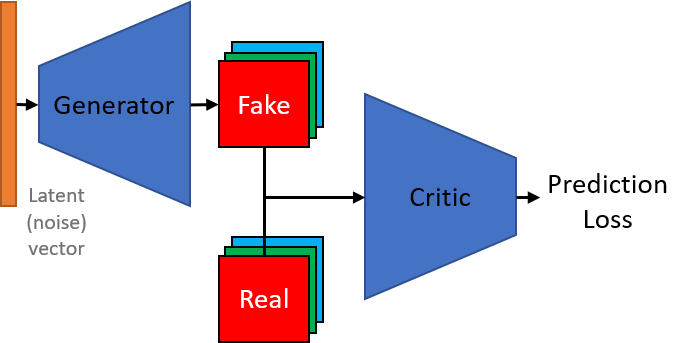
\includegraphics[width=0.5\textwidth]{figures/architecture}
\end{figure}

The hyperparameters are shown in Table~\ref{tab:1} and are generally kept the same as used in their respective original papers and implementations.
\begin{table}[t]
    \centering
    \caption{Hyperparameters for WGAN with GP}
    \label{tab:1}
    \begin{tabular}{l l}
        HYPERPARAMETER               & VALUE \\ [0.5ex]
        \hline
        Adam learning rate           & $0.0001$       \\
        Adam $\beta_1$               & $0.0$          \\
        Adam $\beta_2$               & $0.9$          \\
        Mini-batch size              & $64$           \\
        Input image channels         & $3$            \\
        Input image size             & $64 \times 64$ \\
        Latent features              & $100$          \\
        Critic base features         & $16$           \\
        Generator base features      & $16$           \\
        Critic iterations            & $5$            \\
        Gradient penalty $\lambda{}$ & $10$           \\
        Epochs                       & $500$ \\ [1ex]
    \end{tabular}
\end{table}

To achieve Pegasus-like outputs, the WGAN is trained on the CIFAR-10~\cite{krizhevsky2009cifar10} and STL-10~\cite{coates2011stl10} datasets.
As part of pre-processing, the images are resized to 64x64 pixels and normalised (as required for WGAN convergence).
Finally, all images except those labeled as horses and birds are discarded.
Since WGANs prevent mode collapse, when trained randomly on both horses and birds, the resultant generated images should consist of a combination of horse and bird features.
This works on the hope that a subset of the convolutions will produce horse-like features and another subset will produce bird-like features (wings being the most desirable).
Because of this, it is expected that most outputs will not look like Pegasus, with potentially only a few per 64-batch matching the criteria.



    \section{Results}\label{sec:results}
    Figure~\ref{fig:best-batch} shows the best batch of 64 images:
While most of the samples are very noisy, a horse-like shape can be seen in some samples, and a bird-like shape in others.

Of this batch however, the most Pegasus-like image is shown in Figure~\ref{fig:best-image}.
It has a light colour and, with some imagination, looks like it is flying (with its head in the top left, wings at the top and legs at the bottom).

\begin{figure}[h]
    \centering
    \caption{WGAN architecture}
    \label{fig:best-batch}
    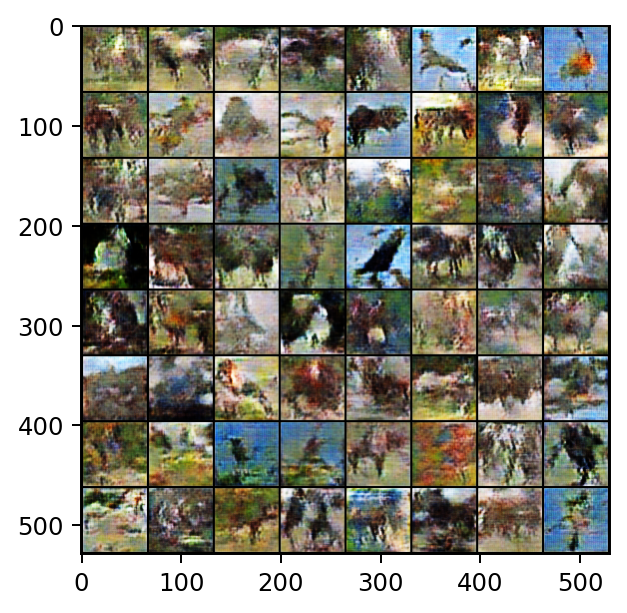
\includegraphics[width=0.5\textwidth]{figures/best-batch}
\end{figure}

\begin{figure}[h]
    \centering
    \caption{WGAN architecture}
    \label{fig:best-image}
    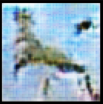
\includegraphics[width=0.075\textwidth]{figures/best-pegasus}
\end{figure}



    \section{Limitations}\label{sec:limitations}
    The majority of the generated images do not look like a Pegasus.
Since the loss converged to around 20 after about 500 epochs, it is unlikely any additional epochs would improve the quality.
Additionally, while improvements would be made with more input image data, the existing CIFAR-10 and STL-10 horse and bird images could be manually curated, choosing those with relevant features (open wings, better matching colours, etc.).

For CIFAR-10 alone, the images tend to converge towards horse-like figures.
Interestingly, for STL-10 alone, the definition is most clear towards the centre of the majority of the images.
Additionally, the sampled images generally look more bird-like than horse-like (of which there are rarely open wings).

Only the labelled images are used, which is a small subset of all the images provided by STL-10.
It may be worth first training a classifier to identify birds and horses so that the rest of the dataset may be used, allowing better learning of the underlying distribution.
This classifier could then potentially be extended to identify birds and horses in the centre of the frame (and even birds with their wings spread).

Potentially, a multi-generator (or even multi-GAN) approach could be used to separately train for bird features and horse features (learning their respective distributions) and sample a linear combination of (manually selected) latent noise vectors which give reasonable results.

Finally, GANs are relatively sensitive to changes in hyperparameter values~\cite{lucic2017gans}.
This means that small changes in their values may result in largely varying results.
With more time, performing a hyperparameter search by either visually inspecting outputs or minimising absolute critic loss would improve results.


    \section*{Bonuses}
    This submission has a total bonus of -3 marks (a penalty), as it uses a GAN and was trained with STL resized to 64x64.

    \printbibliography

\end{document}
